\subsection{Les stratégies de déplacement d'un personnage}

Notre projet inclut des stratégies car les personnages peuvent en effet se déplacer de différentes manières en fonction du contexte ou en fonction du choix de l'utilisateur. Comme le montre le diagramme ci après, chaque stratégie correspond à un type de déplacement (les algorithmes sont expliqués plus loin). \\[0.5cm]

\centerline{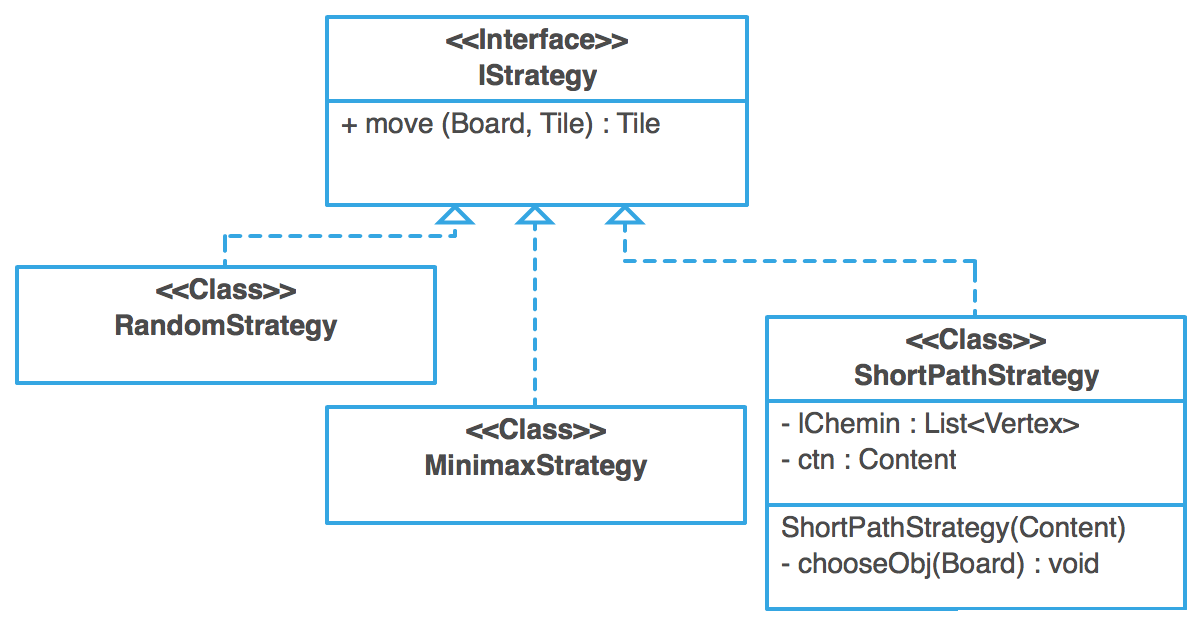
\includegraphics[scale=0.3]{Strategy}}

La méthode move() de chaque stratégie prend en paramètre un Board (cf Gestion des cartes) et une Tile représentant la position courante d'un personnage sur le jeu. La méthode retourne la nouvelle position du personnage.
